\documentclass[]{article}
\usepackage{enumitem}
\usepackage[margin=4cm]{geometry}
\usepackage{indentfirst}
\usepackage[noorphans, vskip=0.6ex]{quoting}
\usepackage{graphicx}
%\usepackage{showframe}
\usepackage[justification=centering]{caption}

\setlength{\parindent}{4em}
\setlength{\parskip}{0.5em}
\renewcommand{\baselinestretch}{1.2}
%opening
\title{Conway's Game of Life and OpenMP\\
\large CITS3402 Programming Assignment 1}
\author{Jesse Wyatt\\20756971}

\begin{document}

\maketitle

\section{Outline}
The purpose of this report is to describe the use of OpenMP to parallelise Conway's Game of Life (GoL), and an analysis of the efficiency of multiple implementations of parallelism as they compare to a serial implementation. As well this report provides a general outline of how to use the supplied code to replicate the results and figures found within.

\section{Setup}
\subsection{Environment}
The code was written for and tested via SSH on an \textit{Ubuntu 18.04 Bionic} virtual machine running in minimal headless mode on an \textit{Intel i7-6700K} (4 physical cores/8 logical cores) with 8 GiB of assigned RAM. The three implementations of the GoL are written in C and were compiled using \textit{GCC 7.3.0} with the default language standard of \texttt{gnu11} and support for \textit{OpenMP 4.5}. Additionally two testing harnesses are provided written for \textit{Python 3.6.5} using the \textit{NumPy} and \textit{Matplotlib} libraries. If using Ubuntu these can be installed easily from a shell prompt with:
\begin{quoting}
	\texttt{sudo apt-get install python3-matplotlib}
\end{quoting}
Otherwise they can be found in several scientific Python distributions such as \textit{Anaconda} and \textit{Canopy}, or installed manually with the Python package manager \texttt{pip}.

\subsection{Usage}
Running either Python harness will automatically compile and run all implementations capturing the output and graphing the results. This can be done from a shell prompt with:
\begin{quoting}
\texttt{python3 infile}
\end{quoting}

\noindent The implementations can also be compiled and run independently with the commands:
\begin{quoting}
\texttt{gcc -fopenmp infile [-o outfile]}

\noindent
\texttt{./outfile [grid\_dimension] [max\_threads]}
\end{quoting}

\noindent Using the variables:
\begin{itemize}[label={}]
\item \texttt{infile} - the path to the source code of the implementation or script
\item \texttt{outfile} - the destination of the compiled binary
\item \texttt{grid\_dimension} - an integer $\lbrace i = n^2 : n \in N \rbrace$  describing the side length of the game grid
\item \texttt{max\_threads} - an integer $\lbrace i : 1 \leq i \leq 32\rbrace$ overriding the number of threads to create
\end{itemize}

\subsection{Source Code}
\noindent The included source files are:
\begin{itemize}[label={}]
\item \texttt{gol\_serial.c} - a simple serial implementation of the GoL

\item \texttt{gol\_parallel.c} - a row-level loop parallelised implementation of the GoL

\item \texttt{gol\_collapse.c} - a collapsed loop parallelised implementation of the GoL

\item \texttt{gol\_benchmark.py} - a script to time and plot benchmarks

\item \texttt{gol\_snapshot.py} - a script to capture and generate snapshots of the game state
\end{itemize}

\section{Output}
If run independently, the GoL implementations will take three snapshots at steps 0, 10, and 20 and will print them to stdout. Each snapshot is separated by a double newline, and consists of \texttt{grid\_dimension} lines of \texttt{grid\_dimension} characters with \texttt{1} indicating an alive cell and \texttt{0} indicating a dead or empty cell.

When the snapshot script is run it will capture stdout and generate a graphical plot of the three snapshots for each implementation with black squares indicating live cell and white squares indicating a dead or empty cell.

When the benchmark script is run it will time each implementation and produce comparative graphs of elapsed real time and equivalent user-space time.

\section{Implementation}
\subsection{General Optimisation}
An effort was made to keep as much of the code as possible between implementations to reduce non-parallelism-related effects on the analysis. As such few simple optimisations are present in all implementations. As the GoL wraps around the edges of the grid modularly, it's necessary to perform modulo operations when indexing into the grid to find neighbours. Unfortunately the default implementation of the "modulus" operator \texttt{\%} in C actually calculates the mathematical remainder which is unsuitable for modular array indexing. Manually implementing a true modulo function can be very inefficient, so acceptable grid dimensions are restricted to powers of 2, allowing a fast bit-flip technique to emulate true modulo:
\begin{quoting}
$\textbf{MOD}(N, M) = N \mathrel{\&}  (M - 1)$
\end{quoting}

Additionally as the state of a cell in the GoL relies on the states of its neighbours in the previous generation the game grid cannot be updated in place, a new grid must be used for each step. For small grid dimensions this isn't an issue, but number of cells grows with the square of grid dimensions so that a grid with a side length of 2048 will contain $2^{22}$ cells, and a naive implementation using integers on a 64-bit system may require up to 32 MiB per grid. To avoid excessive allocation and deallocation Two working arrays are used that swap pointers after each step of the simulation. By swapping pointers the downtime between steps is as short as possible, and as every cell is updated on every step of the simulation there is no need to reinitialise the array.

\subsection{Parallelism}
Most of the control flow and set-up between simulation steps is inherently serial in nature and can't be easily parallelised. The nature of the GoL implies each step must be completed before the next can be started, and imposes natural barriers to pipeline-style parallelism. While each simulation step requires the previous step be completed first, the state of a cell in any particular step is unaffected by the states of its neighbours within that step. This means for each step, cell updates can be performed in any order and are thus a strong candidate for parallelisation. It is also important to note that the status of each cell is calculated in place immediately so there is no need for a reduction process between each simulation step.

For simplicity the cell update process is implemented as a nested loop of row and column indices. Parallelising these loops can be attempted in two ways, either one of the loops can be divided between threads, or by collapsing a series of nested loops into all combinations of loop variables to be divided between threads. Both methods have their own small benefits.

\subsection{Row-level Parallelism}
Only parallelising the outer loop with static scheduling means each thread will be assigned an equal and contiguous share of the backing array. Working with contiguous array segments mean that cache hits are more likely and the solution is potentially more efficient. The loop may also be dynamically scheduled, but as each cell update always requires a fixed number of lookups there is no need for load balancing and we may lose some of the cache efficiency depending on implementation details and race conditions.

\noindent
\texttt{gol\_parallel.c} implements row-level loop parallelism with the compiler directive:

\begin{quoting}
\noindent\texttt{\#pragma omp parallel for private(neighbours)}
\end{quoting}

\subsection{Condensed Loop Parallelism}
In collapsing multiple loops into a series of combinations of loop variables, the compiler creates a single meta-loop and parallises it accordingly. The meta-loop's larger iteration depth reduces the granularity of the work available for assignment, and as such can improve the scalable performance of the parallel segment in cases where there are a high number of threads relative to the iteration depth of the outer loop. Depending on the type of work being performed, collapsing can prevent the compiler from applying appropriate loop nest optimisations, slowing down run time by decreasing cache hits, or by disabling SIMD loop vectorisation.

\noindent
\texttt{gol\_collapse.c} implements collapsed loop parallelism with the compiler directive:

\begin{quoting}
\noindent\texttt{\#pragma omp parallel for collapse(2) private(neighbours)}
\end{quoting}

\section{Analysis}
\subsection{Methodology and Accuracy}
Performing analysis of each implementation that is both efficient and accurate can be difficult as many external factors can affect the run time of a process, including multiple instances of the candidate itself when trying to batch test for averages. This is especially apparent when trying to run the Python harness scripts on low-powered hardware. Python's sluggish memory management results in successive tests progressively slowing down without significant memory overhead. For this reason the provided scripts may produce significantly different results to the figures contained in this report. Graphed results can be compared with either of the \texttt{perf stat}, or \texttt{time} GNU utilities if they are avaliable to verify their accuracy. If analysing the code manually it is useful to also redirect standard output to \texttt{/dev/null} as terminals will typically buffer their displays, potentially slowing down the run time of large simulations by several seconds.

On the testing system the scripts appeared to have very little impact on the final times with results within a few percent to the ideal results produced by 'perf stat', and no progressive slowdown was apparent. For the comparisons between implementation types the maximum threads were left at default values and OpenMP was allowed to dynamically assign threads as it deemed fit.

To demonstrate the accuracy of all implementations the standard library unseeded PRNG was used to initialise the game. As seen in the snapshot plots in the appendix, all simulations evolved consistently. Notably the game state stabilises very quickly with only minor evolution after the 10th generation.

\subsection{Serial Efficiency}
For very small grids of $128^2$ cells or less, the work to complete the core simulation is dwarfed by general system noise and the fork/join processes of OpenMP. For that reason the serial implementation can, in practice, be several times faster than either parallel implementation for small inputs. Although, as the number of cells increases the run time of the serial implementation continues to scale linearly and rapidly surpassess the run time of either parallel solution in practical use.

\begin{figure}[h]
	\centering
	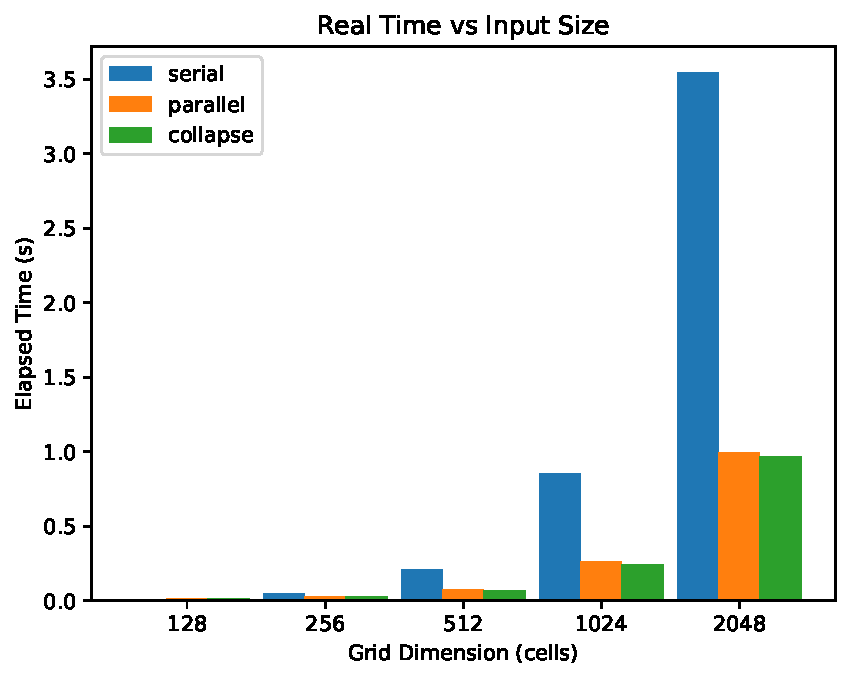
\includegraphics[width=.8\linewidth]{vecs/input_realtime.pdf}
	\caption{Implementation runtimes for grid dimensions.}
\end{figure}

\subsection{Parallel Efficiency}
From the data initially it appears that parallel solutions might somehow scale sub-linearly with the number of cells, as the ratio between average run times of parallel and serial solutions seems to increase with input size. Unfortunately while they are significantly faster, complexity analysis of the parallel solutions shows that they still scale linearly with the number of cells, but with a reduced constant factor. The apparent relative increase in efficiency is a result of the cost of step simulation progressively dominating the overheads of forking and joining. Both implementations of parallelism have produced nearly identical results for the simulation. Parallelising the initial algorithm has not improved its time complexity and this implies there is a narrow region for the usefulness of parallelising the GoL in this way, unless further efficiencies can be found, or computational resources can be scaled alongside input.

\subsection{User Time}
The real time speed improvements of the parallel implementations are also accompanied by a significant increase in resource use and computational complexity. User time is a measurement of how long a processor spends executing code in user-space, and in a multi-threaded system it is the equivalent of all time spent by all threads in a process. By comparing the equivalent time each implementation spends in user-space we can gain an understanding of the amount of pressure being applied to the system, and equivalently an idea of how much energy is being dedicated to the task. When allowing OpenMP to dynamically assign threads on the testing system, it always assigns a thread to each of the 8 logical cores available. Compared to the serial implementation, under these conditions the parallel implementations complete a $2048^2$ cell simulation in roughly 30\% of the time, but with close to double the equivalent time spent in user-space.

\begin{figure}[h]
	\centering
	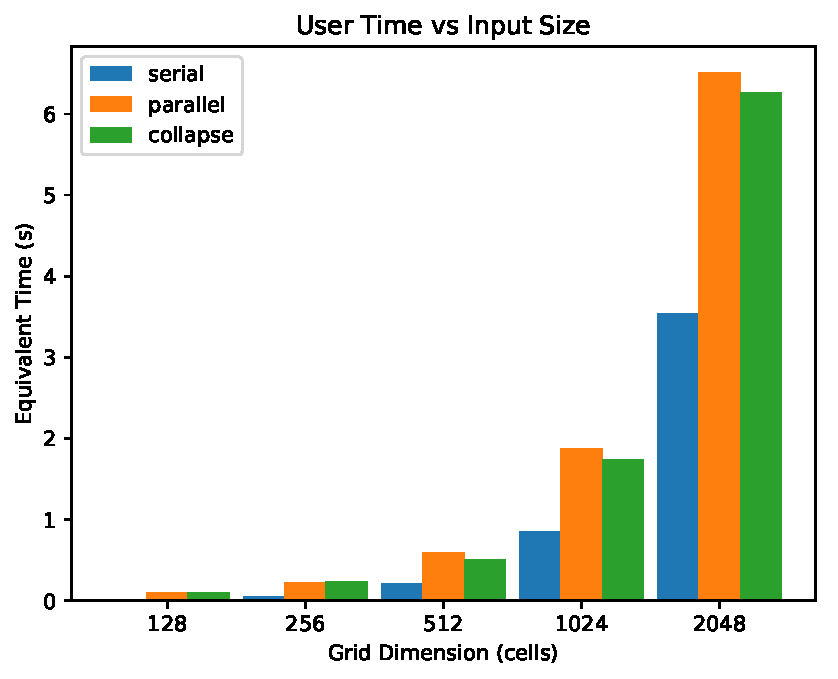
\includegraphics[width=.8\linewidth]{vecs/input_usertime.pdf}
	\caption{Implementation user-space times for grid dimensions.}
\end{figure}

\subsection{Thread Scaling}
Disabling dynamic thread creation and specifying a number of threads allows us to visualise the effect of hyperthreading on our implementations. The real time taken to complete the simulation decreases as threads are added until it plateaus at 8. Notably though, the performance benefit of moving from 4 to 8 threads is minimal and correlates with a large jump in user-space activity. As the testing machine has 4 physical cores and 8 logical cores it appears that generally matching the number of threads to the number of logical cores will give the best real time performance, but in this simulation a majority of the benefit is gained by matching the number of physical cores. As our parallelism is highly regular, with each thread performing an almost identical sequence of computations we can likely conclude that hyperthreading is relatively inefficient when two threads both require use of the same logic units of a single physical core.
\begin{figure}[p]
	\centering
	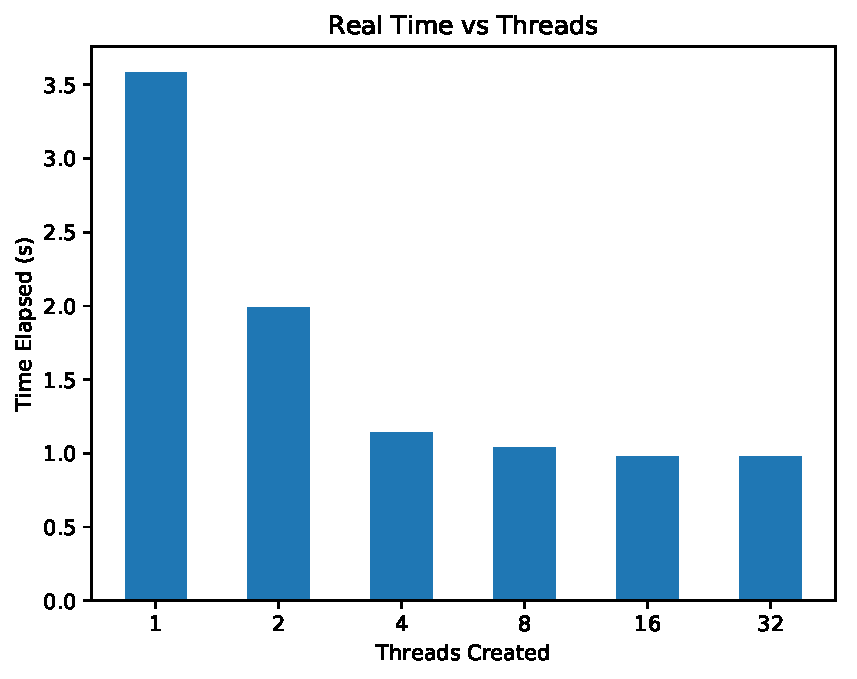
\includegraphics[width=.75\linewidth]{vecs/threads_realtime.pdf}
	\caption{Average runtime for forced thread count row-parallel implementations on a $2048^2$ grid.}
\end{figure}
\begin{figure}[p]
	\centering
	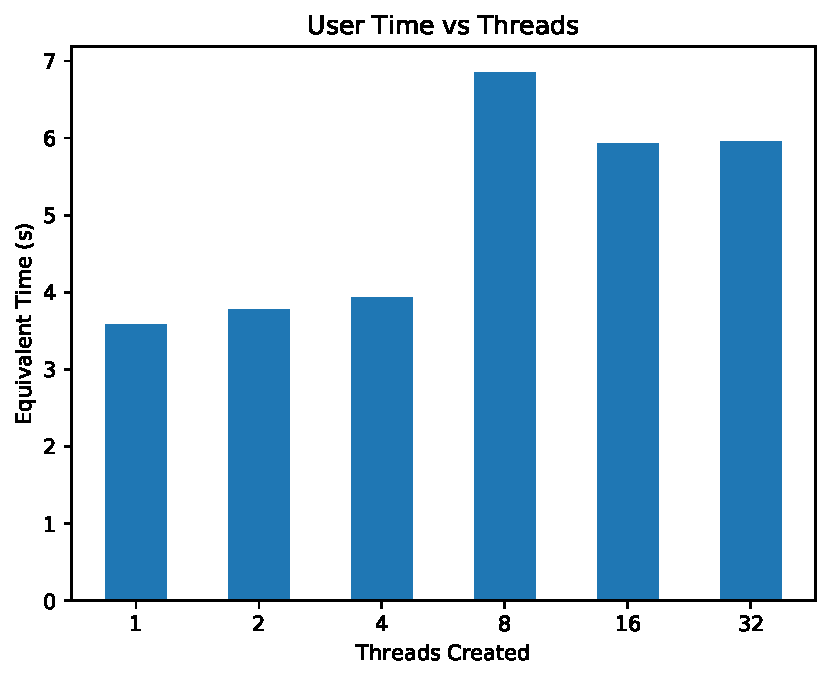
\includegraphics[width=.75\linewidth]{vecs/threads_usertime.pdf}
	\caption{Average user-space time for forced thread count row-parallel implementations on a $2048^2$ grid.}
\end{figure}

\section{Conclusion}
The GoL is relatively simple to parallelise with high levels of scalability, but parallelism alone cannot overcome the polynomial growth of cell count with grid dimensions. There is little apparent difference in the performance of either method of loop parallelism, although collapsed loop methods may scale better on many-core or distributed systems.

It is clear that higher numbers of physical cores are generally beneficial, and performance improves linearly as core count increases. Hyperthreaded logical cores also provide a minor improvement in real time performance, although at a significant increase in system load. In a real-world scenario, where energy consumption and system responsiveness are often important factors it is important to consider if the speed-up of parallelising code of this nature is worthwhile when compared to the increase in resources.

\subsection{Potential Improvements}
Although the nature of the GoL generally prohibits pipeline-style parallelism, there is still potential for a novel implementation if the number of working game grids is scaled up to the number of threads. By delaying each thread until the proceeding thread has completed a specified number of regions, the next state can begin to be calculated before the first state is completed. This method may improve performance by reducing the amount of forks and joins required as the circular nature of the pipeline avoids the need for swapping out grids at each step. Issues with this implementation are that it could be potentially difficult to extract individual complete states from the pipeline, and the reliance on the first threads completing their work before their successors catch up introduce the risk of race conditions, especially as caching may provide an uneven performance benefit to the successor thread. To avoid race conditions each thread must communicate with the others at regular intervals which can add significant overhead costs.


\section{Appendix}
The following appendix contains snapshots of all implementations in all valid sizes ranging between 128 to 2048.

\subsection{128x128}
\begin{center}
	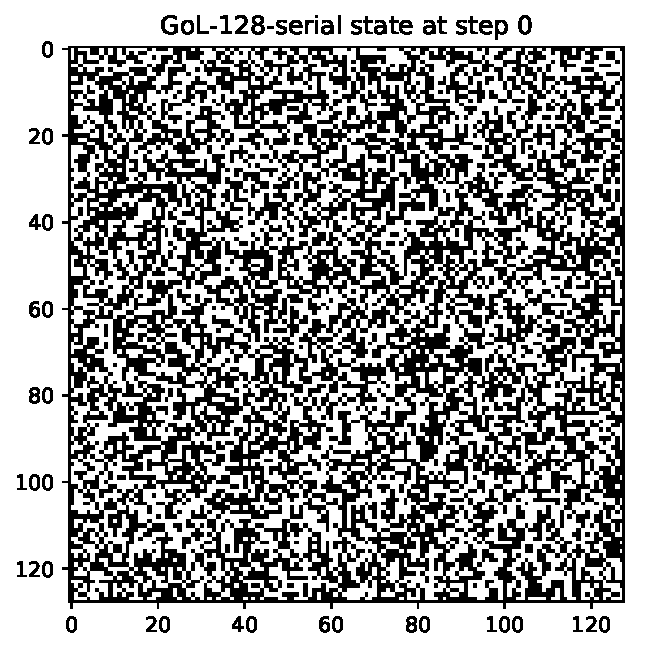
\includegraphics[width=.3\linewidth]{vecs/serial128_0.pdf}
	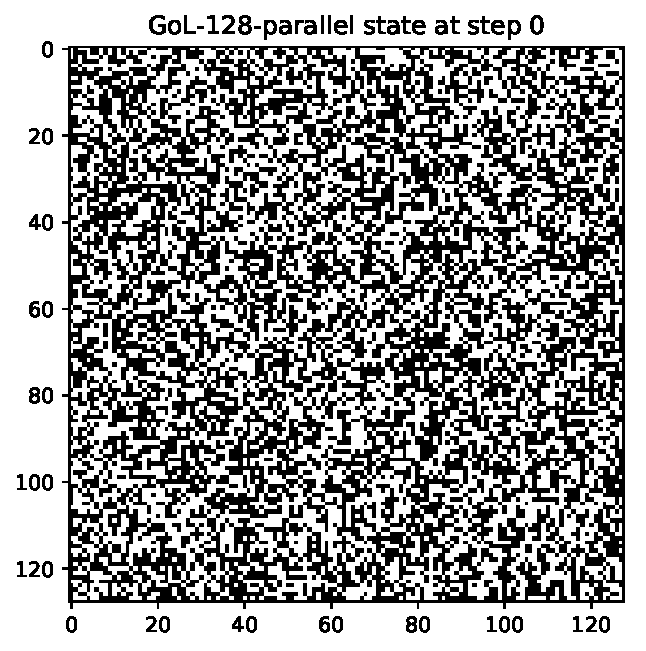
\includegraphics[width=.3\linewidth]{vecs/parallel128_0.pdf}
	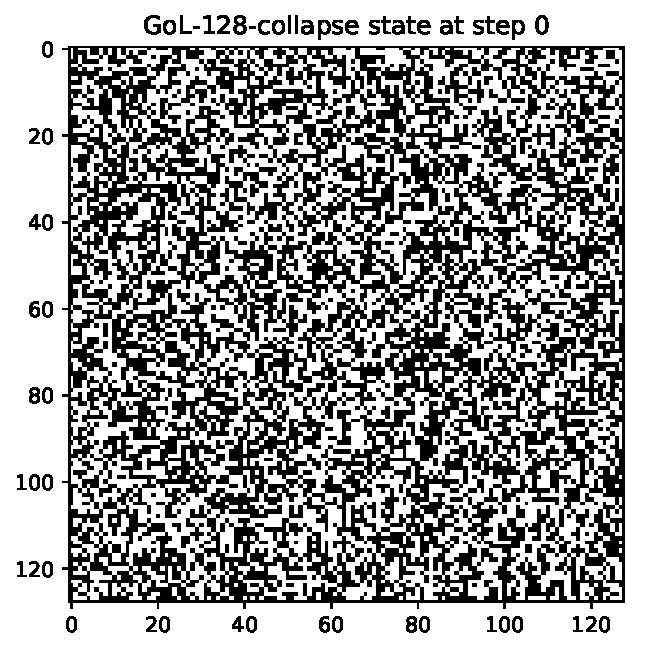
\includegraphics[width=.3\linewidth]{vecs/collapse128_0.pdf}\\
	[\baselineskip]
	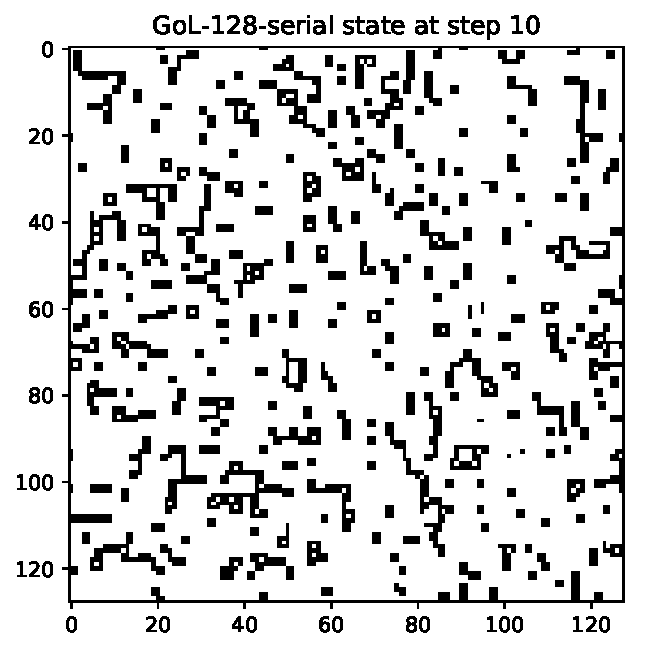
\includegraphics[width=.3\linewidth]{vecs/serial128_10.pdf}
	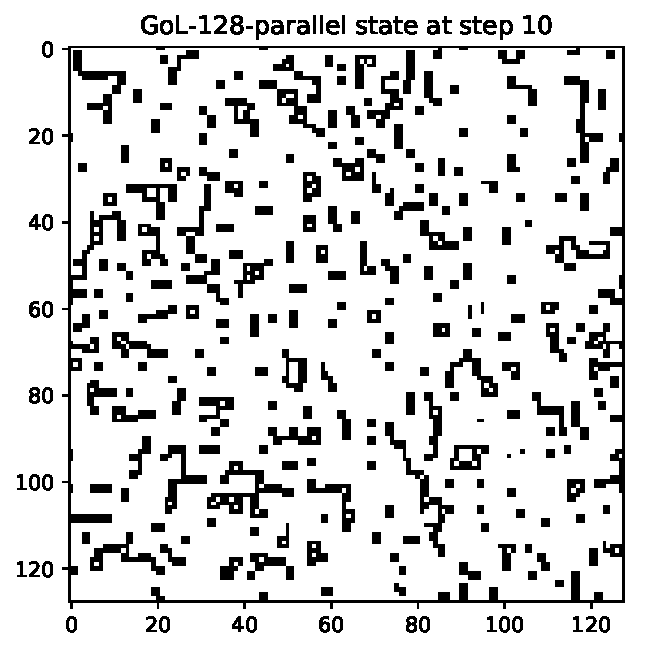
\includegraphics[width=.3\linewidth]{vecs/parallel128_10.pdf}
	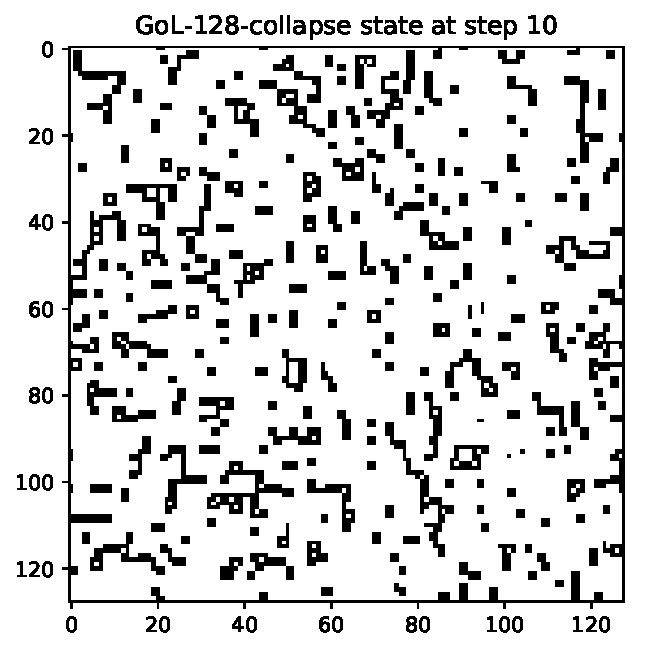
\includegraphics[width=.3\linewidth]{vecs/collapse128_10.pdf}\\
	[\baselineskip]
	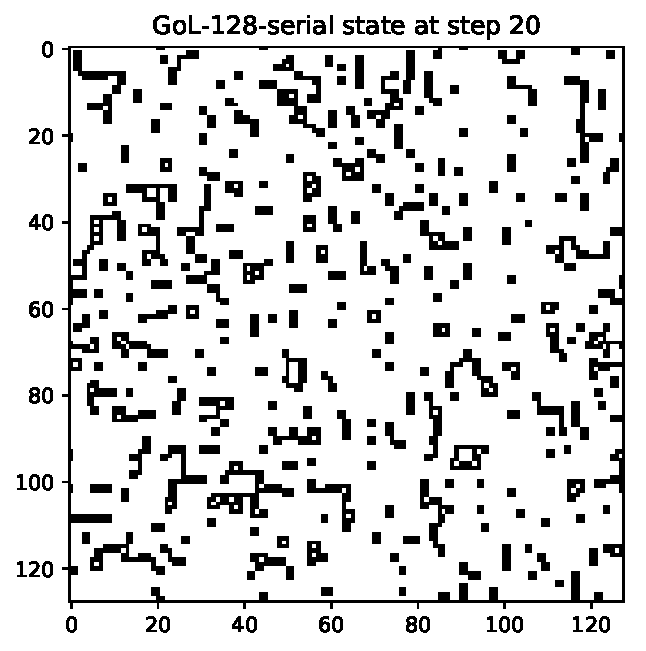
\includegraphics[width=.3\linewidth]{vecs/serial128_20.pdf}
	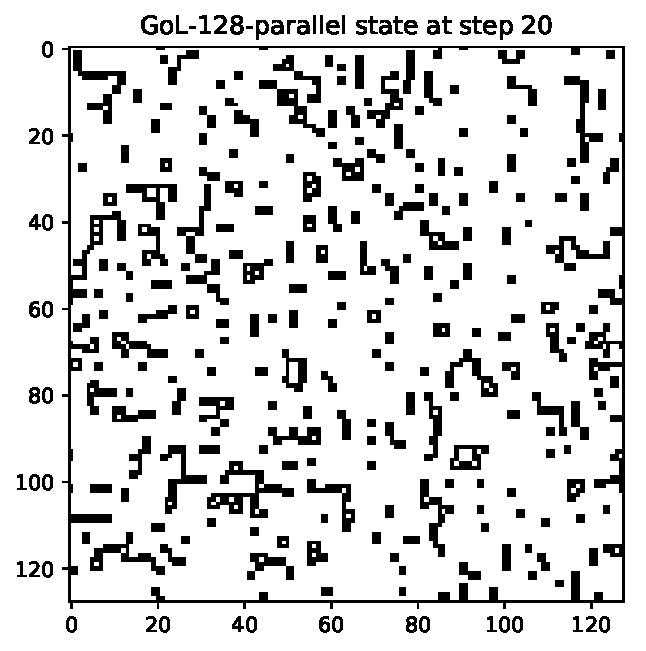
\includegraphics[width=.3\linewidth]{vecs/parallel128_20.pdf}
	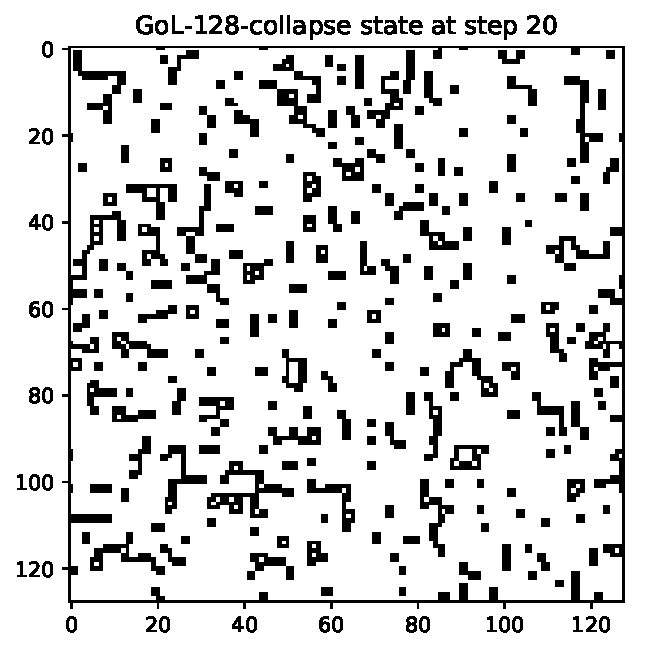
\includegraphics[width=.3\linewidth]{vecs/collapse128_20.pdf}\\
\end{center}
\newpage

\subsection{256x256}
\begin{center}
	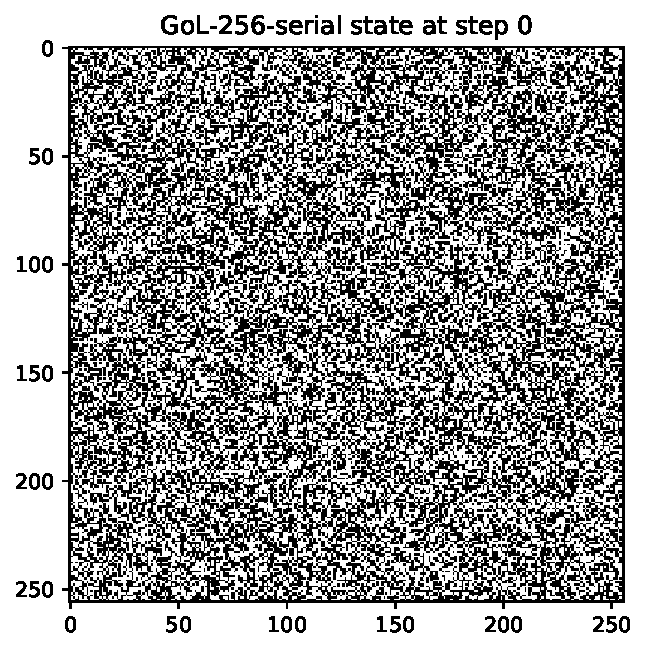
\includegraphics[width=.3\linewidth]{vecs/serial256_0.pdf}
	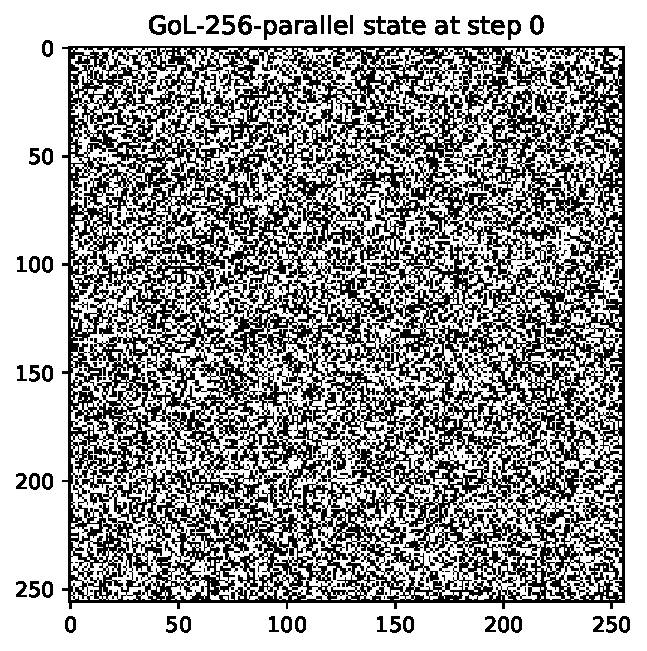
\includegraphics[width=.3\linewidth]{vecs/parallel256_0.pdf}
	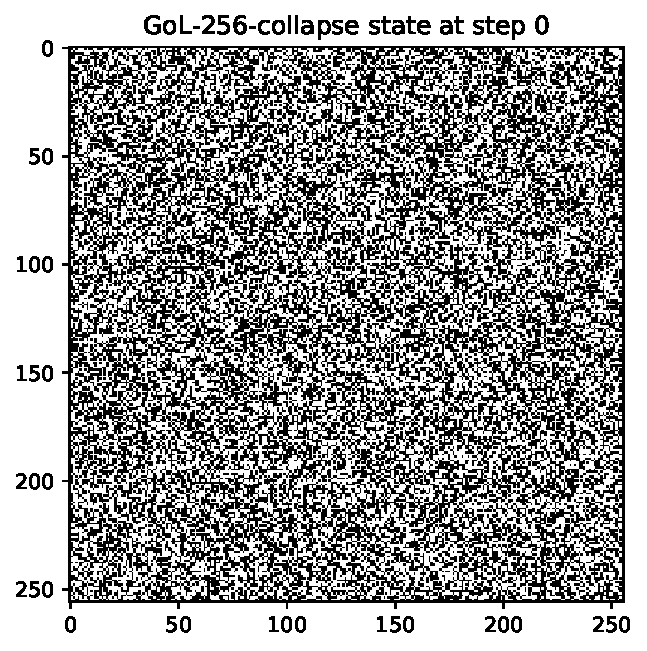
\includegraphics[width=.3\linewidth]{vecs/collapse256_0.pdf}\\
	[\baselineskip]
	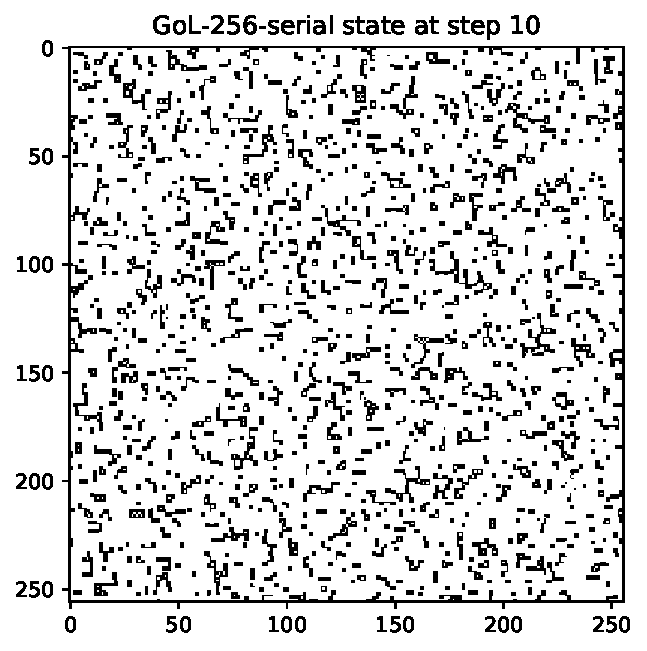
\includegraphics[width=.3\linewidth]{vecs/serial256_10.pdf}
	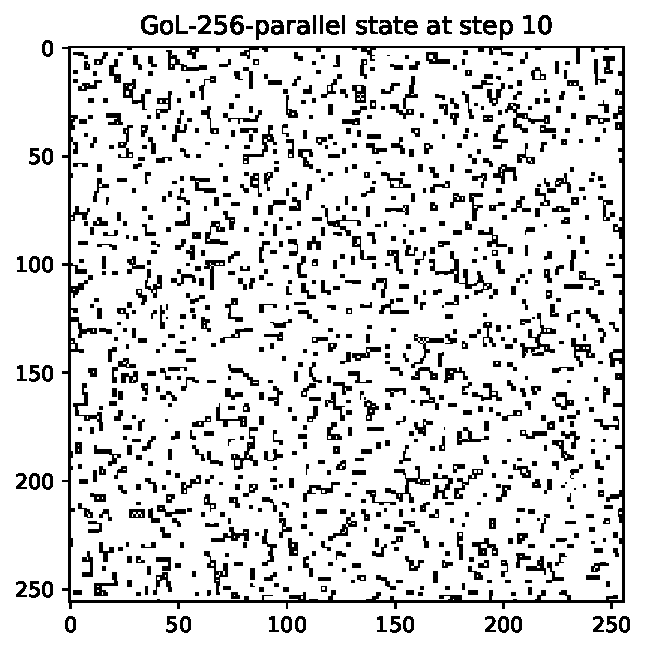
\includegraphics[width=.3\linewidth]{vecs/parallel256_10.pdf}
	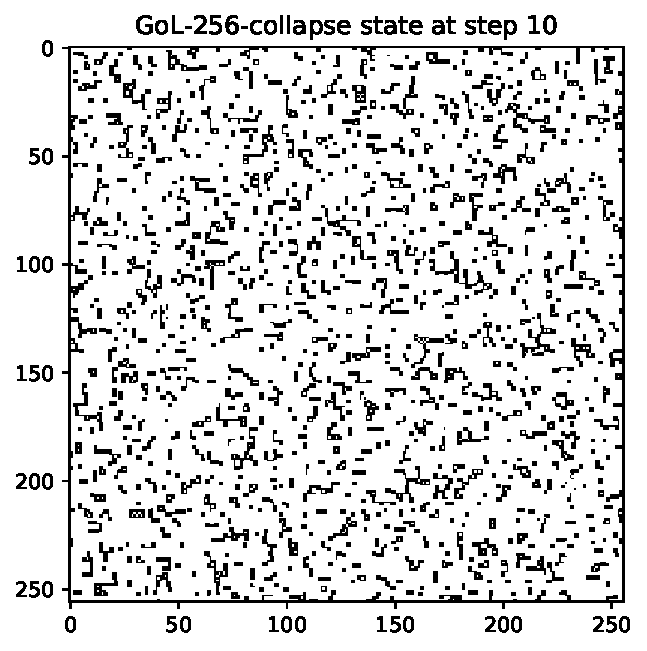
\includegraphics[width=.3\linewidth]{vecs/collapse256_10.pdf}\\
	[\baselineskip]
	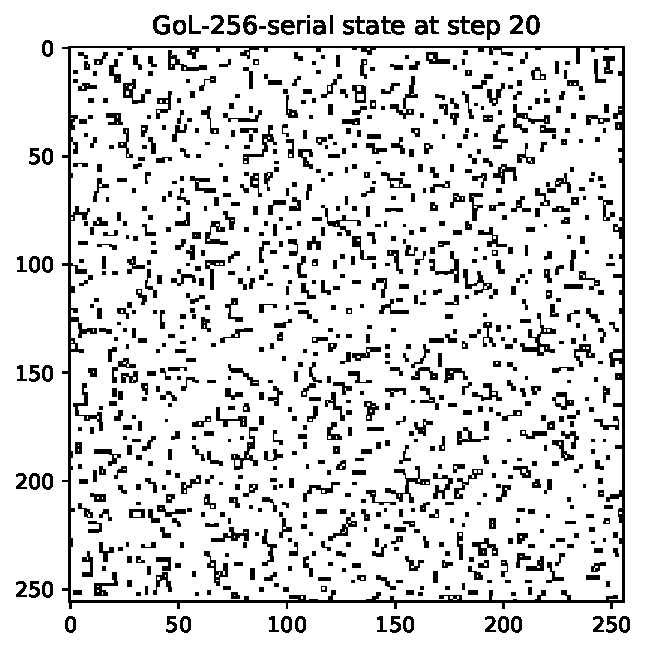
\includegraphics[width=.3\linewidth]{vecs/serial256_20.pdf}
	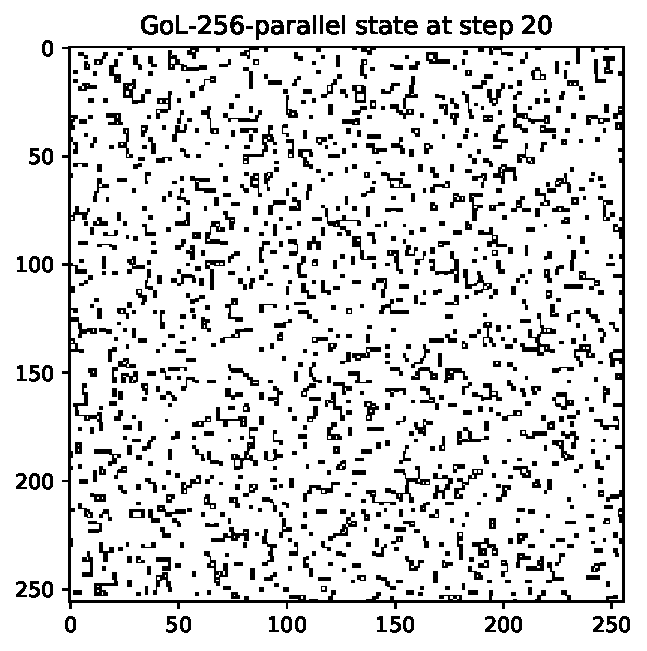
\includegraphics[width=.3\linewidth]{vecs/parallel256_20.pdf}
	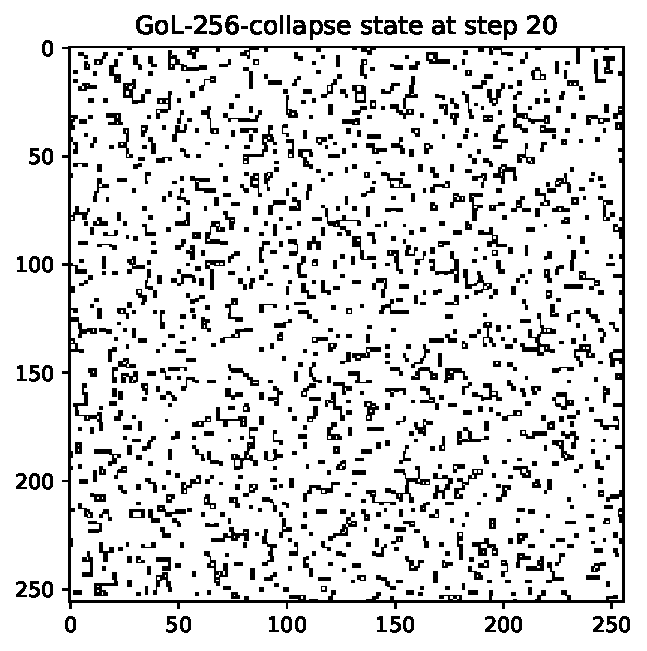
\includegraphics[width=.3\linewidth]{vecs/collapse256_20.pdf}\\
\end{center}
\newpage

\subsection{512x512}
\begin{center}
	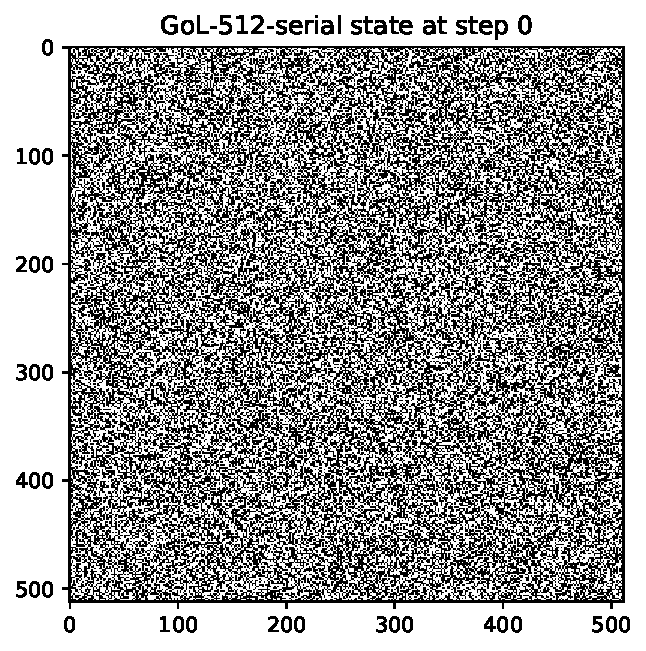
\includegraphics[width=.3\linewidth]{vecs/serial512_0.pdf}
	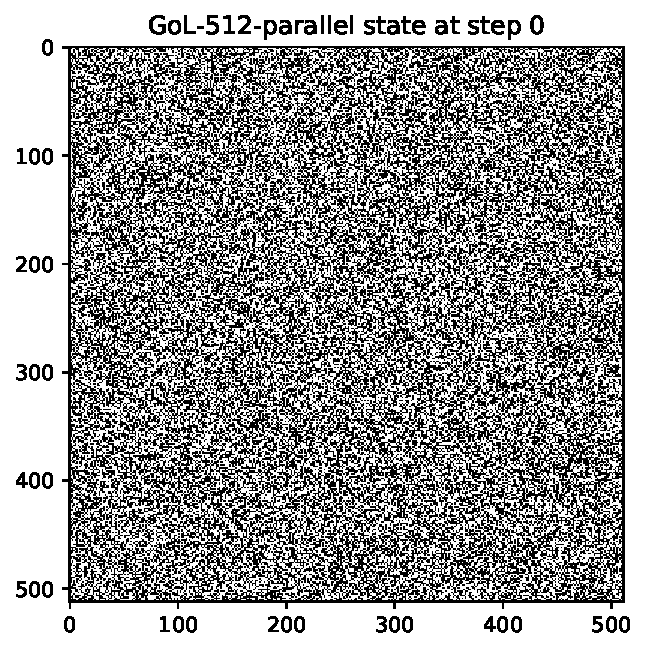
\includegraphics[width=.3\linewidth]{vecs/parallel512_0.pdf}
	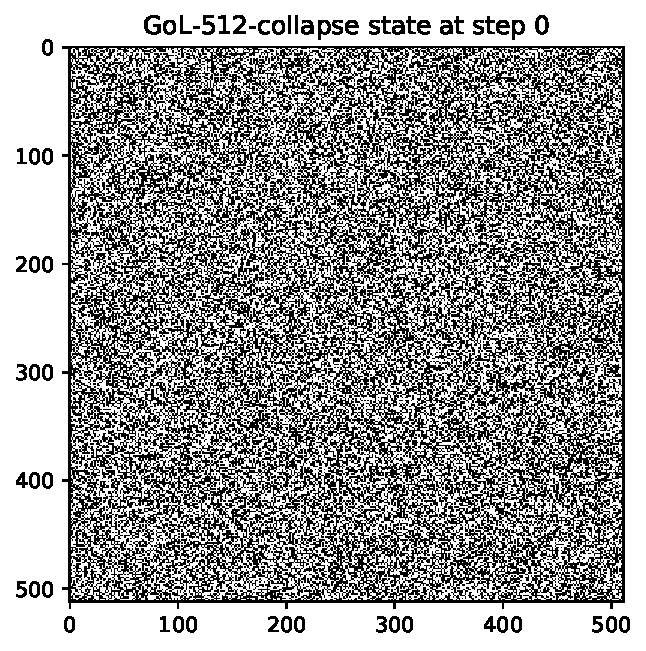
\includegraphics[width=.3\linewidth]{vecs/collapse512_0.pdf}\\
	[\baselineskip]
	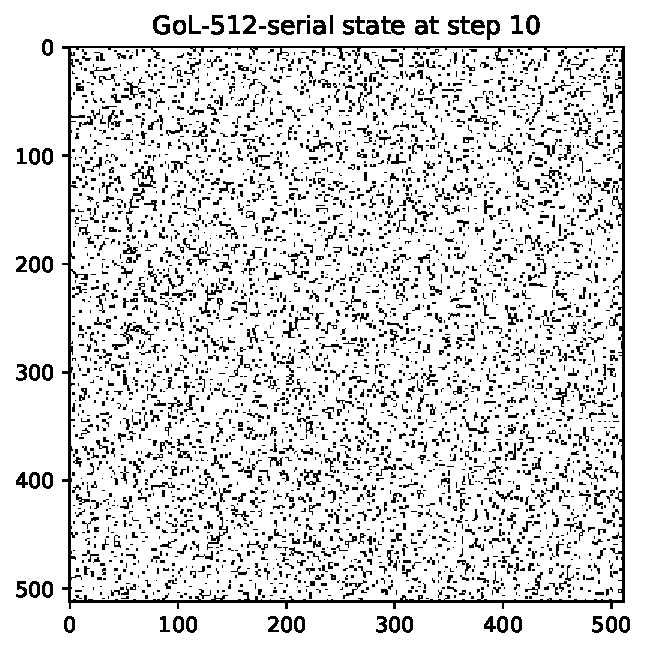
\includegraphics[width=.3\linewidth]{vecs/serial512_10.pdf}
	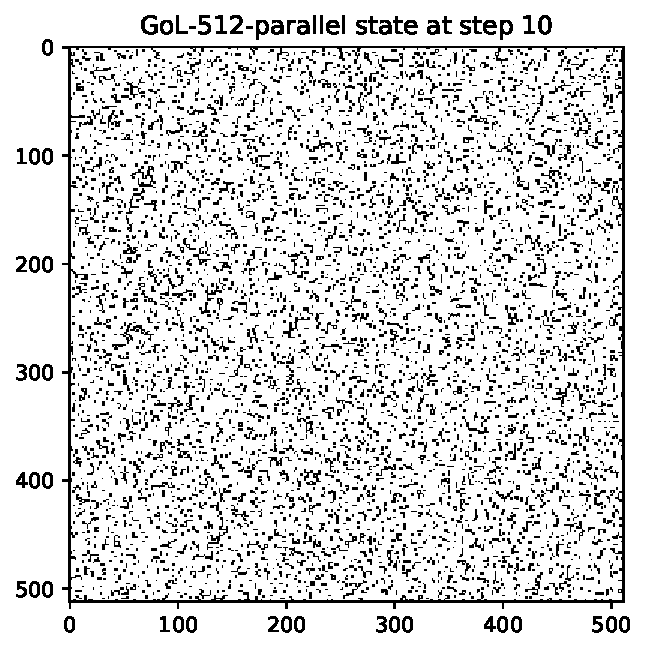
\includegraphics[width=.3\linewidth]{vecs/parallel512_10.pdf}
	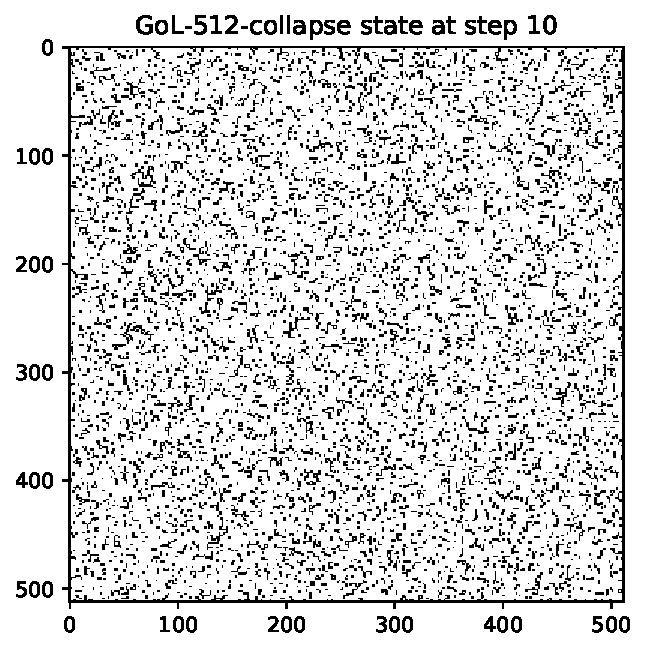
\includegraphics[width=.3\linewidth]{vecs/collapse512_10.pdf}\\
	[\baselineskip]
	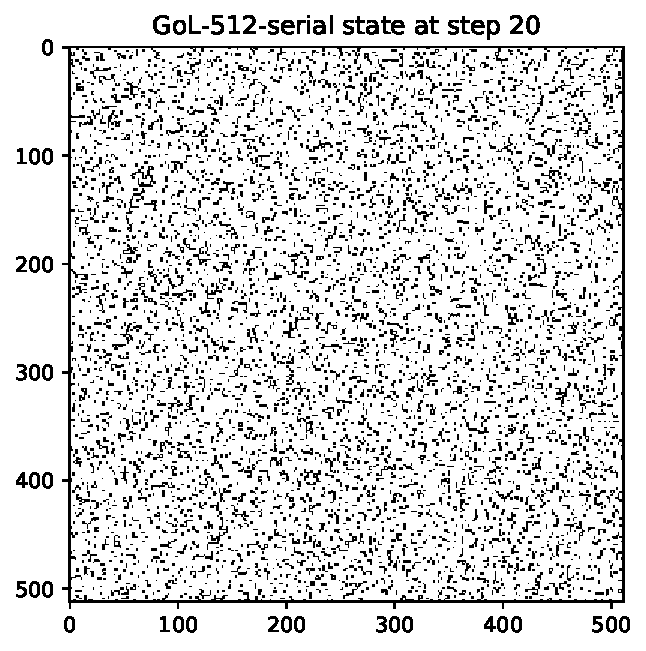
\includegraphics[width=.3\linewidth]{vecs/serial512_20.pdf}
	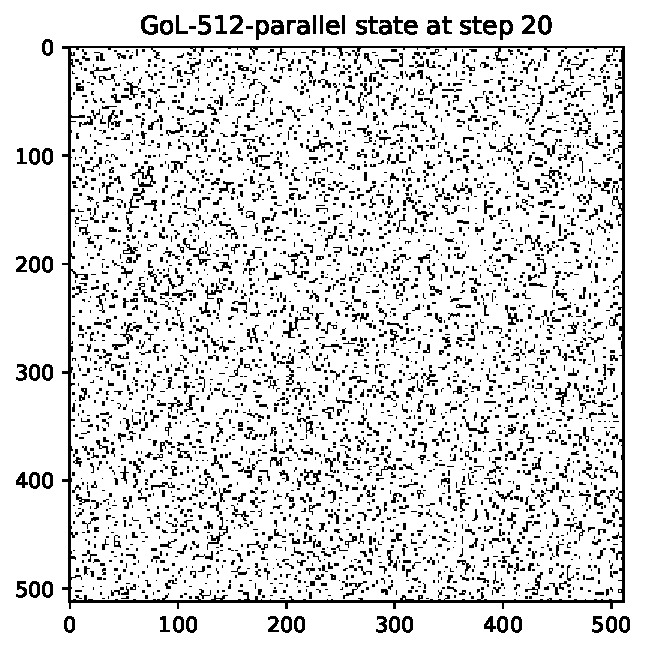
\includegraphics[width=.3\linewidth]{vecs/parallel512_20.pdf}
	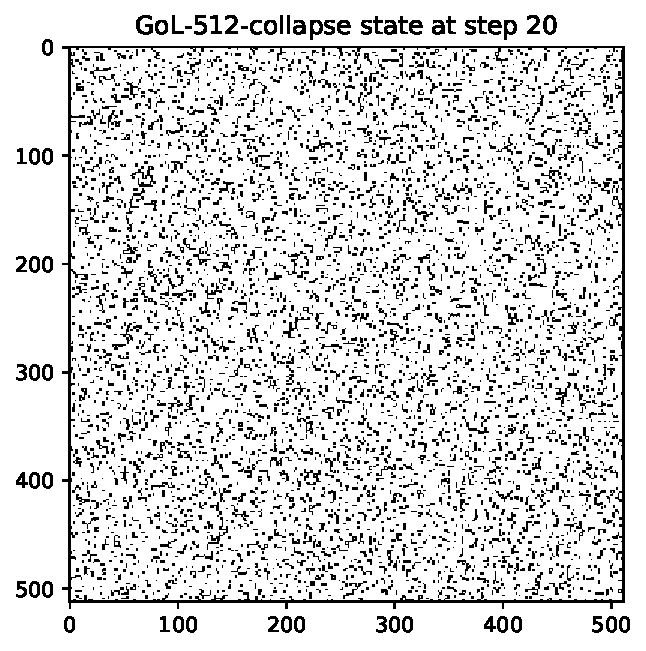
\includegraphics[width=.3\linewidth]{vecs/collapse512_20.pdf}\\
\end{center}
\newpage

\subsection{1024x1024}
\begin{center}
	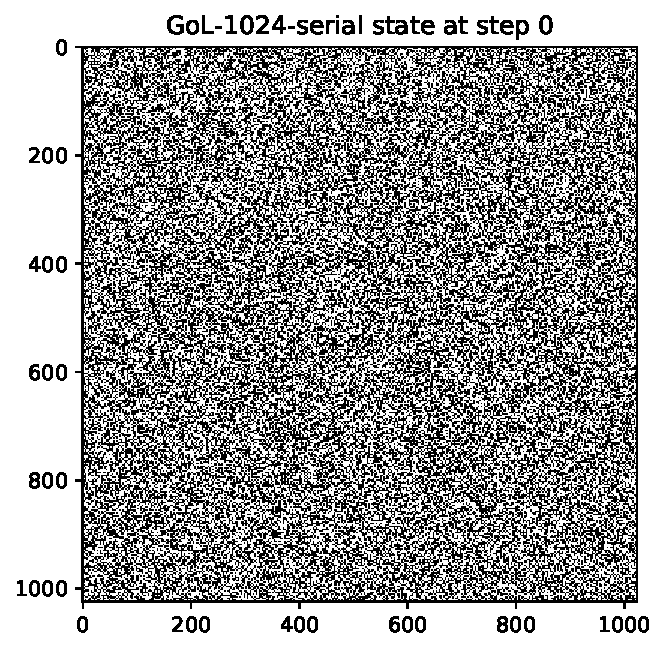
\includegraphics[width=.3\linewidth]{vecs/serial1024_0.pdf}
	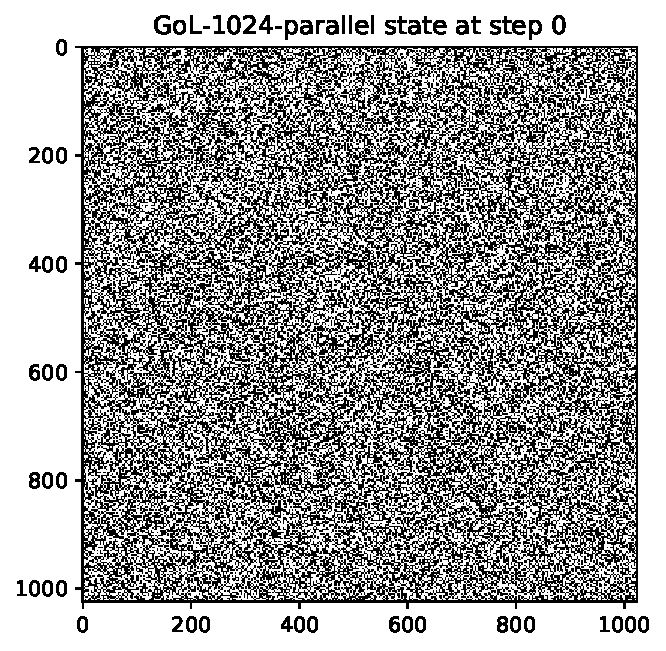
\includegraphics[width=.3\linewidth]{vecs/parallel1024_0.pdf}
	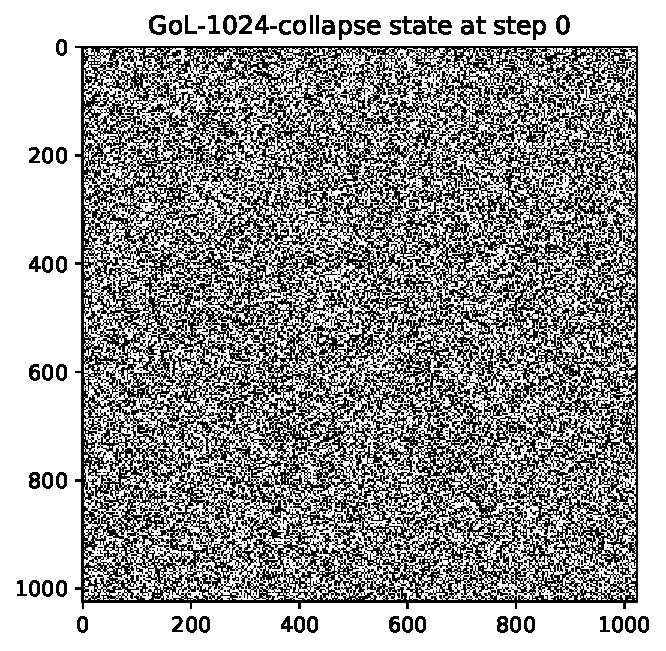
\includegraphics[width=.3\linewidth]{vecs/collapse1024_0.pdf}\\
	[\baselineskip]
	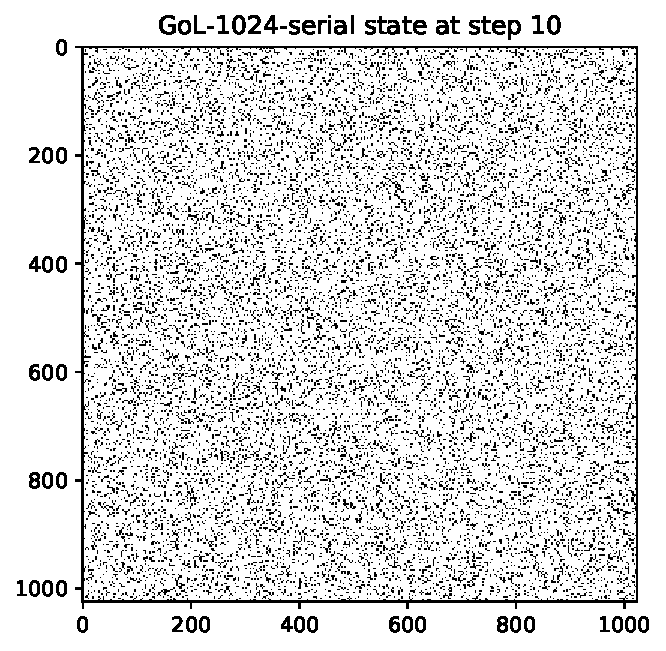
\includegraphics[width=.3\linewidth]{vecs/serial1024_10.pdf}
	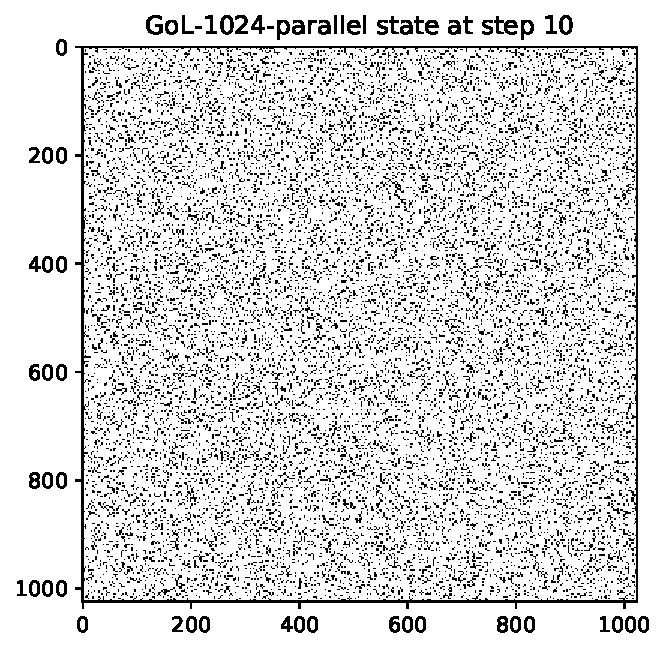
\includegraphics[width=.3\linewidth]{vecs/parallel1024_10.pdf}
	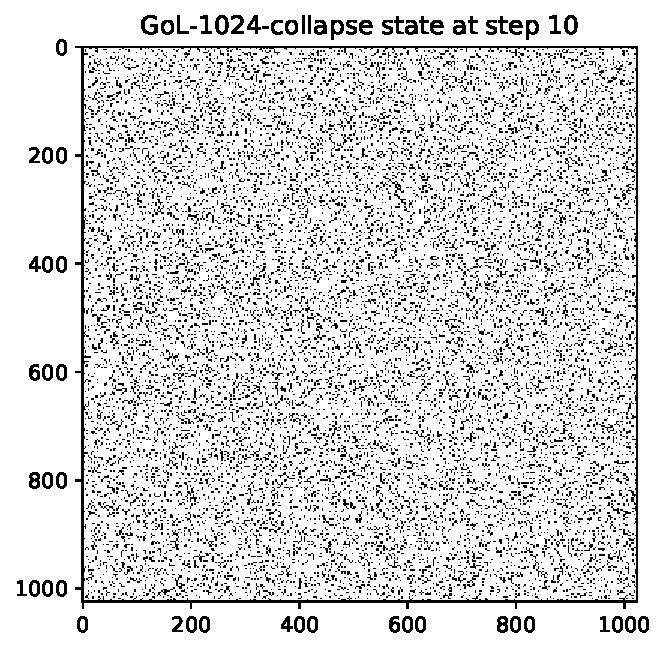
\includegraphics[width=.3\linewidth]{vecs/collapse1024_10.pdf}\\
	[\baselineskip]
	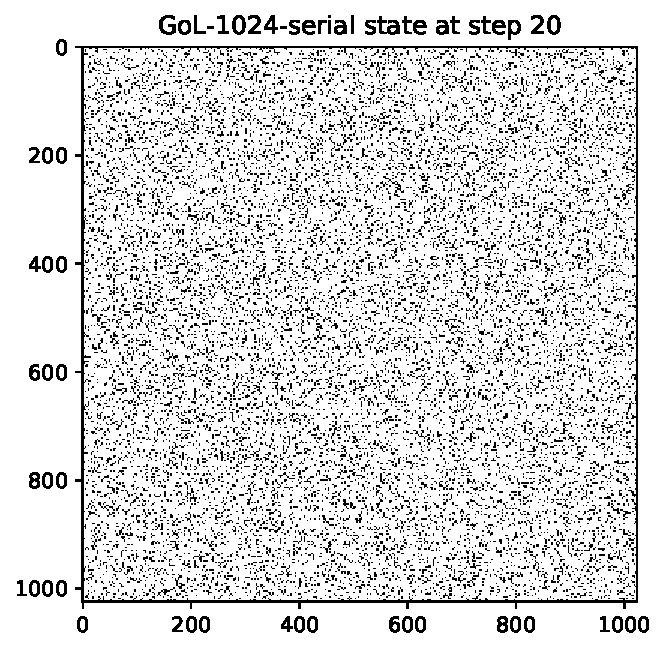
\includegraphics[width=.3\linewidth]{vecs/serial1024_20.pdf}
	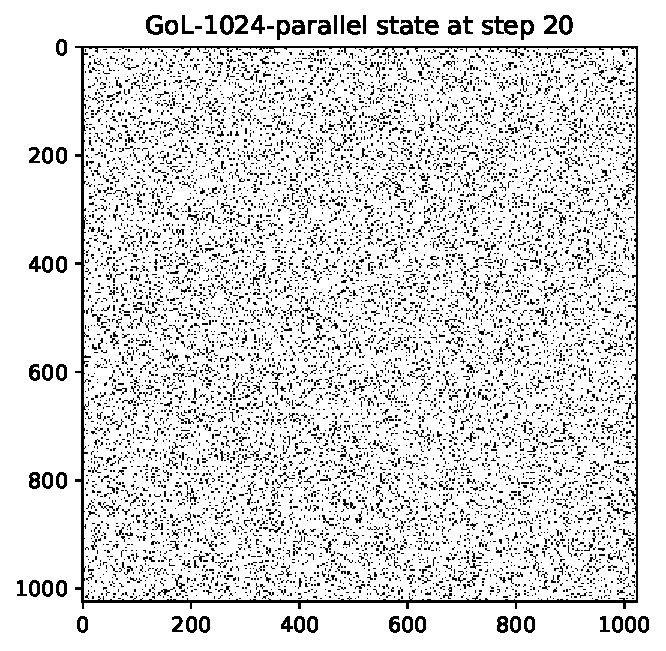
\includegraphics[width=.3\linewidth]{vecs/parallel1024_20.pdf}
	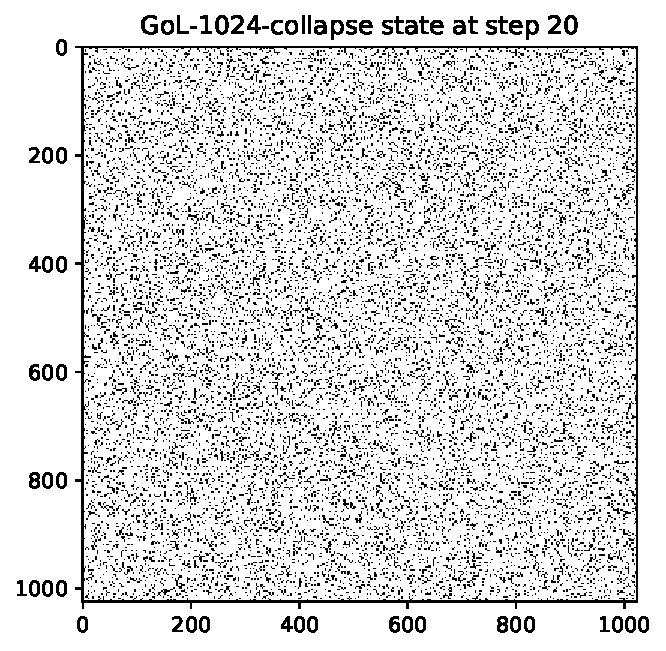
\includegraphics[width=.3\linewidth]{vecs/collapse1024_20.pdf}\\
\end{center}
\newpage

\subsection{2048x2048}
\begin{center}
	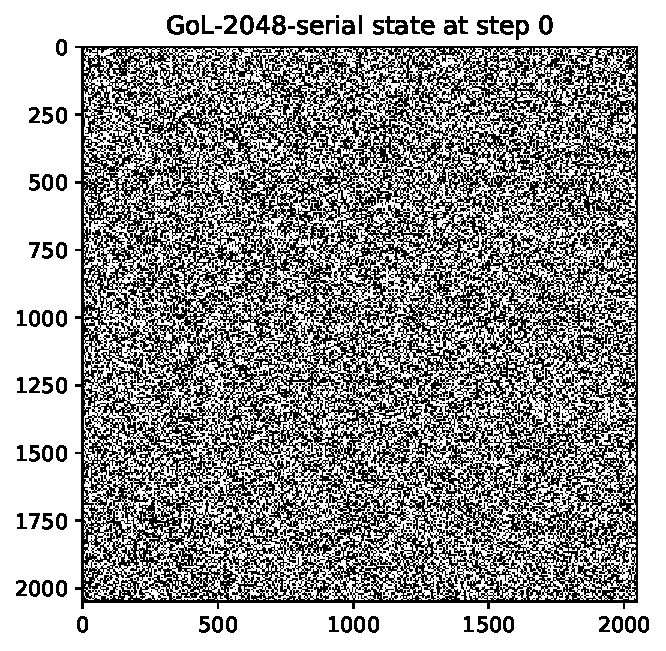
\includegraphics[width=.3\linewidth]{vecs/serial2048_0.pdf}
	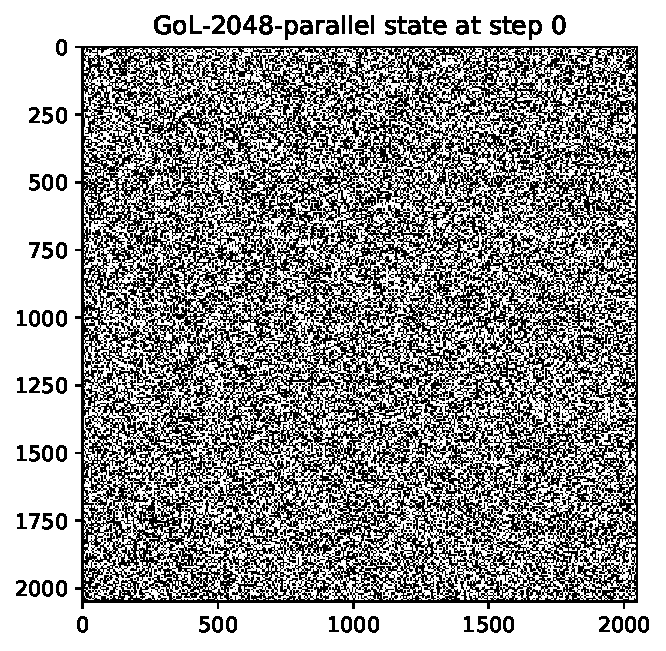
\includegraphics[width=.3\linewidth]{vecs/parallel2048_0.pdf}
	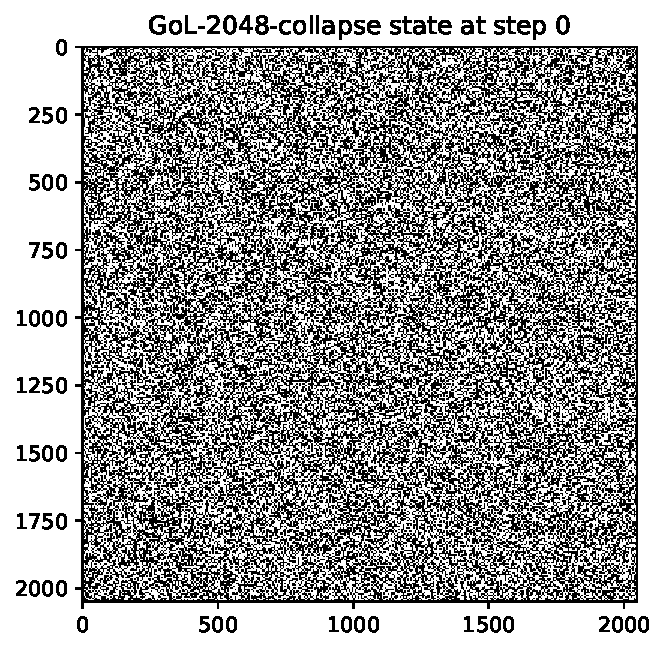
\includegraphics[width=.3\linewidth]{vecs/collapse2048_0.pdf}\\
	[\baselineskip]
	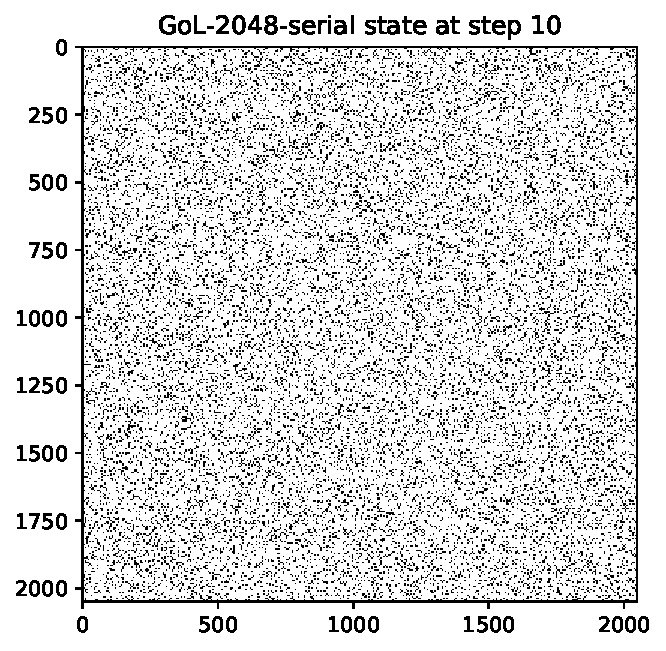
\includegraphics[width=.3\linewidth]{vecs/serial2048_10.pdf}
	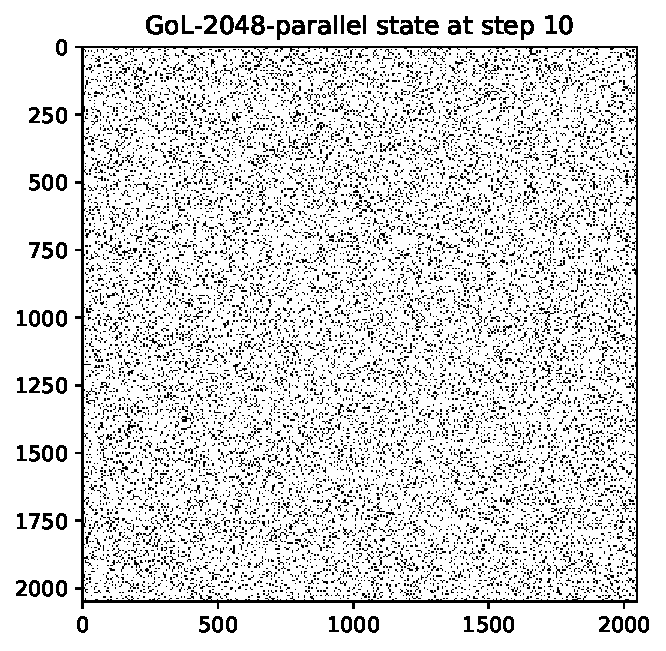
\includegraphics[width=.3\linewidth]{vecs/parallel2048_10.pdf}
	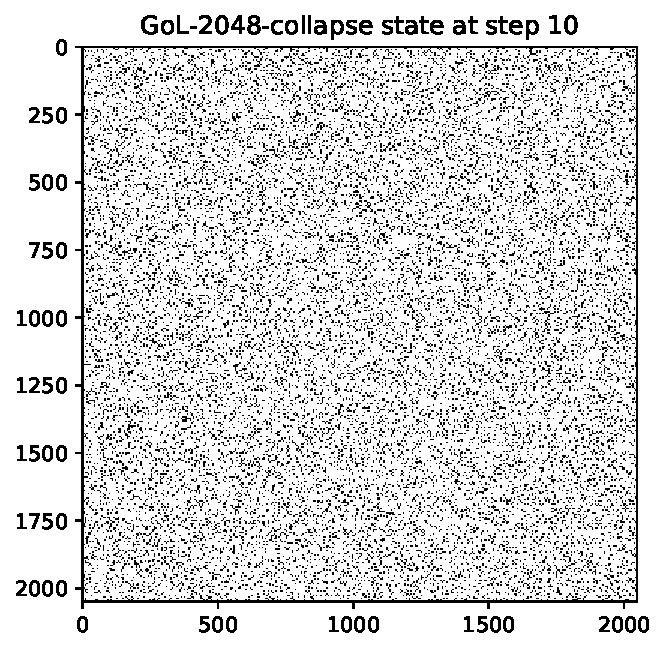
\includegraphics[width=.3\linewidth]{vecs/collapse2048_10.pdf}\\
	[\baselineskip]
	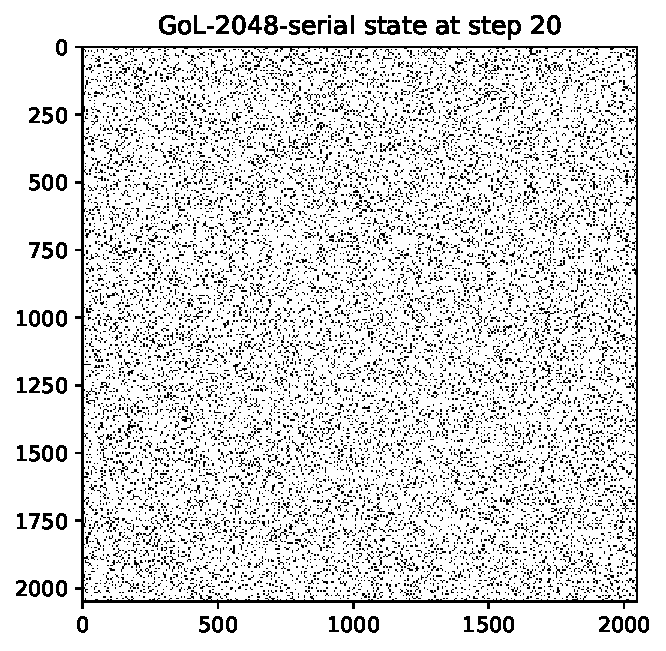
\includegraphics[width=.3\linewidth]{vecs/serial2048_20.pdf}
	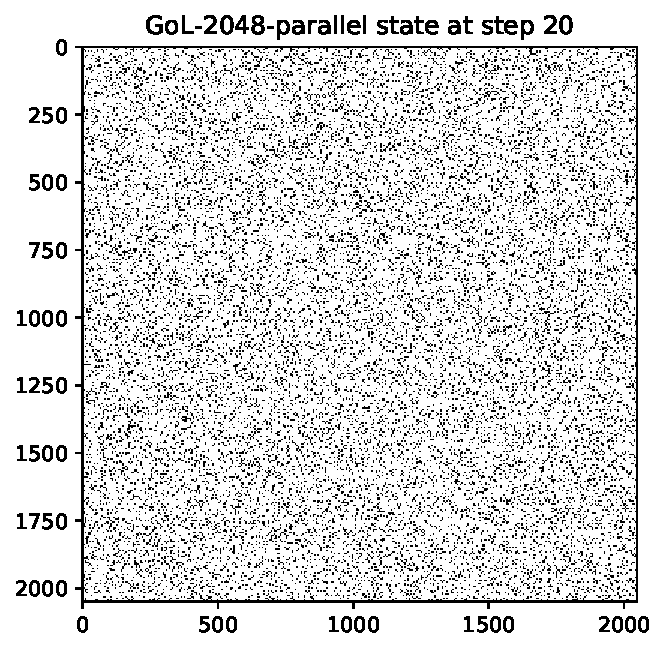
\includegraphics[width=.3\linewidth]{vecs/parallel2048_20.pdf}
	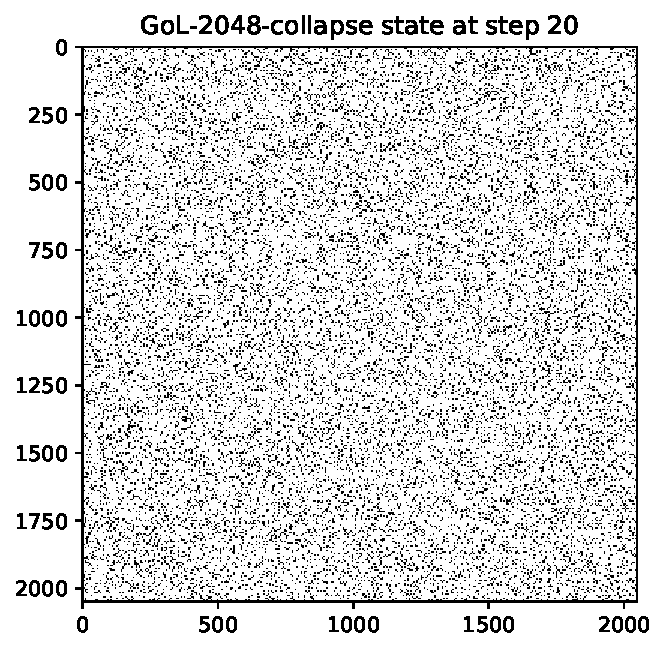
\includegraphics[width=.3\linewidth]{vecs/collapse2048_20.pdf}\\
\end{center}

\end{document}
